\subsubsection{Time Convolution Property}

We rewrite the left hand side (convolution in time domain) using the definition of the Fourier transform 
\begin{equation}
    \begin{aligned}
        \mathcal{F}(x_1 * x_2)\left( w \right) &= \mathcal{F} \left( \int_{-\infty}^{\infty} x_1(\tau) x_2(t - \tau) d\tau \right) \\
        &= \int_{-\infty}^{\infty}  \left( \int_{-\infty}^{\infty} x_1(\tau) x_2(t - \tau) d\tau \right) e^{-2\pi i w t} dt \\
    \end{aligned}
\end{equation}

Next, assuming that $x_1, x_2 \in L_1(\R)$ then we have:

\begin{equation}
    \begin{aligned}
        \int_{-\infty}^{\infty}\int_{-\infty}^{\infty} \sizeof{ x_1(\tau) x_2(t - \tau) e^{-2\pi i w t} } d\tau dt &= \int_{-\infty}^{\infty}\int_{-\infty}^{\infty} \sizeof{ x_2(t - \tau)} dt \sizeof{ x_1(\tau)} d\tau \\
        & =  \norm{x_2}_1 \int_{-\infty}^{\infty} \sizeof{ x_1(\tau)} d\tau \\
        &= \norm{x_1}_1 \norm{x_2}_1
    \end{aligned}
\end{equation}

So by Fubini's theorem we have that:

\begin{equation}
    \begin{aligned}
        \int_{-\infty}^{\infty}  \left( \int_{-\infty}^{\infty} x_1(\tau) x_2(t - \tau) d\tau \right) e^{-2\pi i w t} dt &= \int_{-\infty}^{\infty}  \left( \int_{-\infty}^{\infty} x_2(t - \tau) e^{-2\pi i w t}  dt \right) x_1(\tau) d \tau \\
        &= \int_{-\infty}^{\infty}  X_2(w) \cdot e^{-2\pi i w \tau} x_1(\tau) d \tau \\
        &= X_2(w) \cdot X_1(w)
    \end{aligned}
\end{equation}


\subsubsection{Linearity Property}

\begin{equation}
    \begin{aligned}
        \mathcal{F}(a x_1 + b x_2)\left( w \right) &= \int_{-\infty}^{\infty} \left( a x_1(\tau) + b x_2(\tau) \right) e^{-2\pi i w \tau} d\tau \\
        &= \int_{-\infty}^{\infty} a x_1(\tau) e^{-2\pi i w \tau} + b x_2(\tau) e^{-2\pi i w \tau} \; d\tau \\
        &= a X_1(w) + b X_2(w)
    \end{aligned}
\end{equation}


\subsubsection{Scaling Property}

\begin{equation}
    \begin{aligned}
        \mathcal{F}(x_1(at)) &= \int_{-\infty}^{\infty} x_1(a\tau) e^{-2\pi i w \tau} d\tau \\
        &= \int_{-\infty}^{\infty} x_1(\tau') e^{-2\pi i w \frac{\tau'}{a}} \cdot \frac{1}{a} d\tau' \\
        &= \frac{1}{a} X_1\left(\frac{w}{a} \right)
    \end{aligned}
\end{equation}


\subsubsection{Time Shifting Property}

\begin{enumerate}
    \item  \begin{equation}
        \begin{aligned}
            \mathcal{F}(x_1(t - t_0)) &= \int_{-\infty}^{\infty} x_1(\tau - t_0) e^{-2\pi i w \tau} d\tau \\
            &= \int_{-\infty}^{\infty} x_1(\tau') e^{-2\pi i w \left( \tau' + t_0 \right)} d\tau' \\
            &= X_1\left(w \right) \cdot e^{-2\pi i w t_0}
        \end{aligned}
    \end{equation}

    \item Time shifting has \textbf{no} effect on the amplitude spectrum.
    \item Time shifting causes a linear phase shift of $2\pi w$

\end{enumerate}

\subsubsection{Fourier Transform of rect Function}
\begin{enumerate}
    \item We compute the Fourier transform by definition and scaling property:
    \begin{equation}
        \begin{aligned}
            \mathcal{F}\left(\text{rect}\left( \frac{x}{\tau} \right)\right) &= \int_{-\infty}^{\infty} \text{rect}\left( \frac{x}{\tau} \right) e^{-i \omega x} dx \\
            &= \int_{-\frac{\tau}{2}}^{\frac{\tau}{2}} 1 \cdot e^{- i \omega x} dx \\
            &= \frac{1}{ i \omega} \left( e^{- i \omega \frac{\tau}{2}} - e^{- i \cdot \left( -\frac{\tau}{2} \right)} \right) \\
            &= \frac{2}{\omega} \sin\left( \frac{\omega \tau}{2} \right) \\
            &= \tau \, \text{sinc} \left( \frac{\omega \tau}{2} \right)
        \end{aligned}
    \end{equation}

    \item We attach Figure 7.10 from B.P Lathi which contains the required plots.
    \begin{figure}[h]
        \centering
        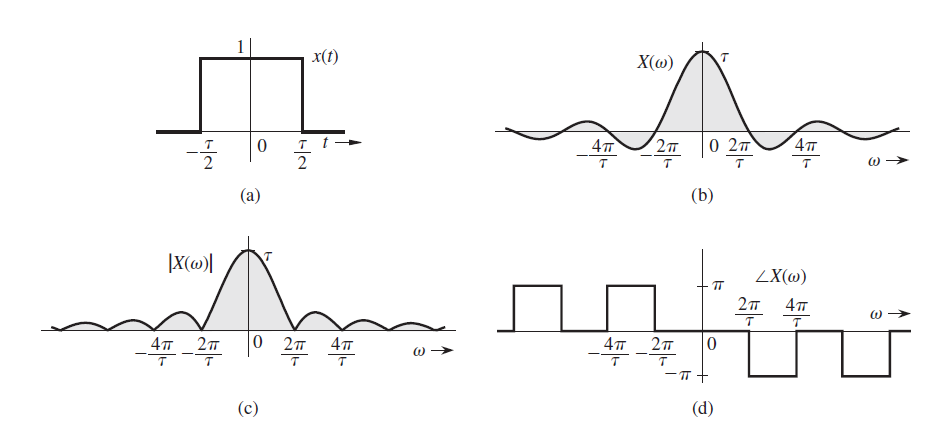
\includegraphics[width=0.78\textwidth]{rec.png}
    \end{figure}

\end{enumerate}

\subsection{Fourier Series}

\subsubsection{Fourier Series of The Delta Function}
\begin{enumerate}
  \item Note that $\delta_{T_0}(t)$ is $T_0$-periodic function, we compute its Fourier coefficients:

  \begin{equation} \label{eq:train_coeff}
    \begin{aligned}
        D_n &= \frac{1}{T_0} \int_{-\frac{T_0}{2}}^{\frac{T_0}{2}} \delta_{T_0}(t) e^{- \frac{2\pi}{T_0} i n t} dt \\
        &= \frac{1}{T_0} e^{- \frac{2\pi}{T_0} i n \cdot 0} \\
        &= \frac{1}{T_0}
    \end{aligned}
  \end{equation}
  where the second equality is by definition (sampling property) of the Dirac Delta function.

  \item We attach Figure 6.15 from B.P Lathi which contains the required plots.
    \begin{figure}[h]
        \centering
        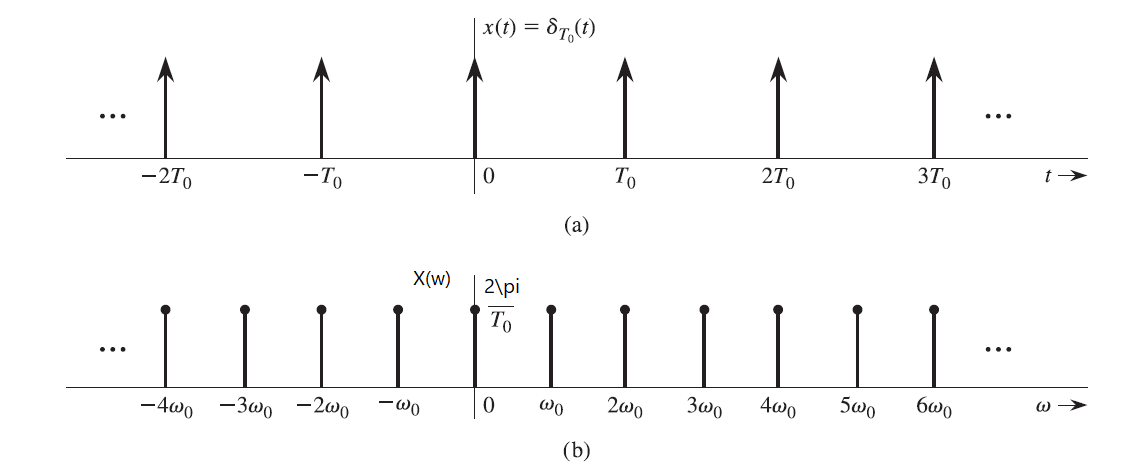
\includegraphics[width=0.78\textwidth]{train.png}
    \end{figure}

    \item $T_0$ is the period of the the impulse train given in question.

    \item Because $\delta_{T_0}(t)$ is $T_0$-periodic, we know that the frequency corresponding to the $n$-th coefficient is $\frac{2\pi}{T_0}n$
      so the interval in frequency space between $D_{n+1}$ and $D_n$ is $\frac{2\pi}{T_0}$.

\end{enumerate}

\subsection{Periodic rect Function}

Notice that by section a.5 the function $x$ drawn in the figure is the $2\pi$ periodic continuation of the function $\text{rect}\left(\frac{t}{\pi}\right) \big|_{[-\pi, \pi]}$.
As seen in class this function can be expressed as a convolution with the corresponding impulse train:
\begin{equation}
  x = \text{rect}\left(\frac{\cdot}{\pi}\right) * \delta_{2\pi}
\end{equation}

By the convolution theorem we have that
\begin{equation}
  \begin{aligned}
    \left(\mathcal{F}x\right)(\omega) &= \mathcal{F}\left( \text{rect}\left(\frac{\cdot}{\pi}\right) \right) \cdot \mathcal{F}\left(\delta_{2\pi}\right) \\
    &= \pi \, \text{sinc}\left(\frac{\pi \omega}{2}\right) \cdot \delta_{1}(\omega)
  \end{aligned}
\end{equation}
We attach Figure 6.6 from B.P Lathi which contains the amplitude plot with sign representing the phase:
\begin{figure}[h]
  \centering
  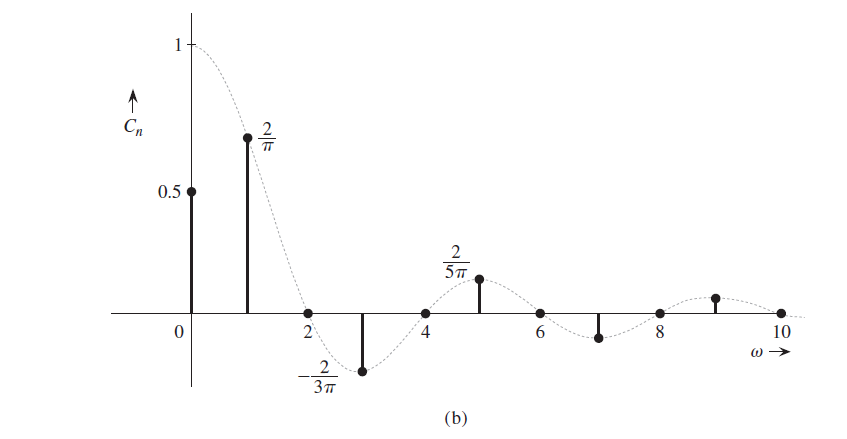
\includegraphics[width=0.78\textwidth]{sampled_sinc.png}
\end{figure}

\subsection{Heaviside Step Function}
\begin{enumerate}
  \item 
    \begin{equation}
      \begin{aligned}
        \left(\mathcal{F}x\right)(\omega) &= \int_{-\infty}^{\infty} u(\tau) e^{-a \tau -i \omega \tau} \\
        &= \int_{0}^{\infty} e^{-\left(a + i \omega\right)\tau} \\
        &= -\frac{1}{a + \omega i} \left(0 - 1\right) \\
        &= \frac{1}{a + \omega i} \\
        &= \frac{a }{a^2 + \omega^2} - \frac{\omega}{a^2 + \omega^2} i
      \end{aligned}
    \end{equation}
    
    \item For the purpose of plotting with chose $a=1$.
    \begin{figure}[h]
      \centering
      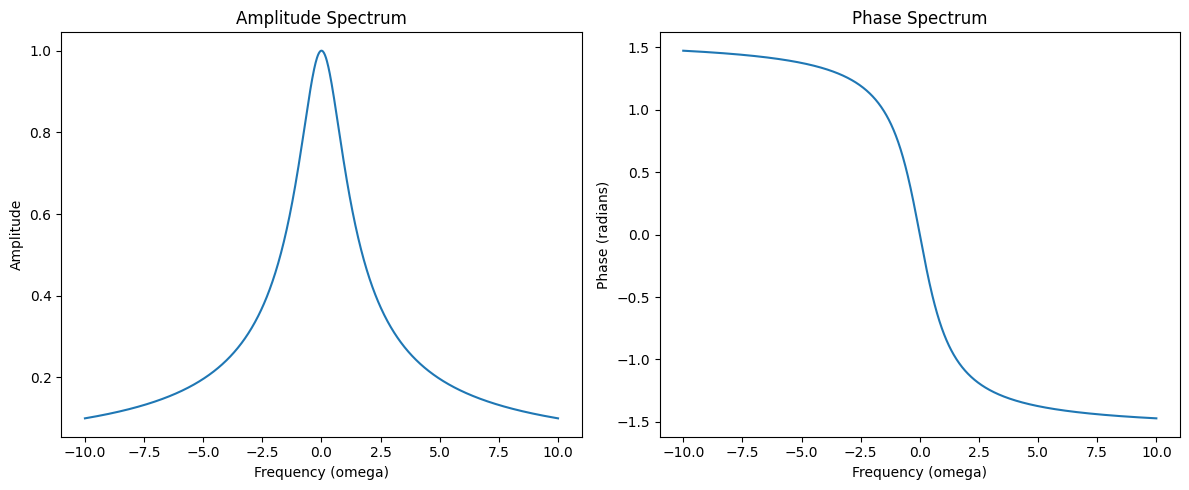
\includegraphics[width=0.9\textwidth]{from_gpt.png}
    \end{figure}

    \item Note that the amplitude spectrum of $X$ decays quadratically with the frequency, so by the convolution theorem $x$ could be used as a \textbf{low} pass filter.   
\end{enumerate}






